\documentclass{beamer}

\usefonttheme{professionalfonts} % using non standard fonts for beamer
\usefonttheme{serif} % default family is serif

\usepackage{hyperref}
%\usepackage{minted}
\usepackage{animate}
\usepackage{graphicx}
\def\Put(#1,#2)#3{\leavevmode\makebox(0,0){\put(#1,#2){#3}}}
\usepackage{color}
\usepackage{tikz}
\usepackage{amssymb}
\usepackage{enumerate}


\newcommand\blfootnote[1]{%

  \begingroup

  \renewcommand\thefootnote{}\footnote{#1}%

  \addtocounter{footnote}{-1}%

  \endgroup

}

\makeatletter

%%%%%%%%%%%%%%%%%%%%%%%%%%%%%% Textclass specific LaTeX commands.

 % this default might be overridden by plain title style

 \newcommand\makebeamertitle{\frame{\maketitle}}%

 % (ERT) argument for the TOC

 \AtBeginDocument{%

   \let\origtableofcontents=\tableofcontents

   \def\tableofcontents{\@ifnextchar[{\origtableofcontents}{\gobbletableofcontents}}

   \def\gobbletableofcontents#1{\origtableofcontents}

 }

%%%%%%%%%%%%%%%%%%%%%%%%%%%%%% User specified LaTeX commands.

\usetheme{Malmoe}

% or ...

\useoutertheme{infolines}

\addtobeamertemplate{headline}{}{\vskip2pt}

\setbeamercovered{transparent}

% or whatever (possibly just delete it)

\makeatother

\begin{document}
\title[PFLOCK report]{PFLOCK Report}
\author[AC]{Andres Calderon}
\institute[Summer'19]{University of California, Riverside}
\makebeamertitle
\newif\iflattersubsect

\AtBeginSection[] {
    \begin{frame}<beamer>
    \frametitle{Outline} 
    \tableofcontents[currentsection]  
    \end{frame}
    \lattersubsectfalse
}

\AtBeginSubsection[] {
    \begin{frame}<beamer>
    \frametitle{Outline} 
    \tableofcontents[currentsubsection]  
    \end{frame}
}

\begin{frame}{LA\_10K Maximal disks finding}
    $\mu=5, \delta=15$.\\
    \blfootnote{Number of flocks: 5134}
    \centering
    \begin{figure}
        \begin{minipage}[b]{0.48\textwidth}
            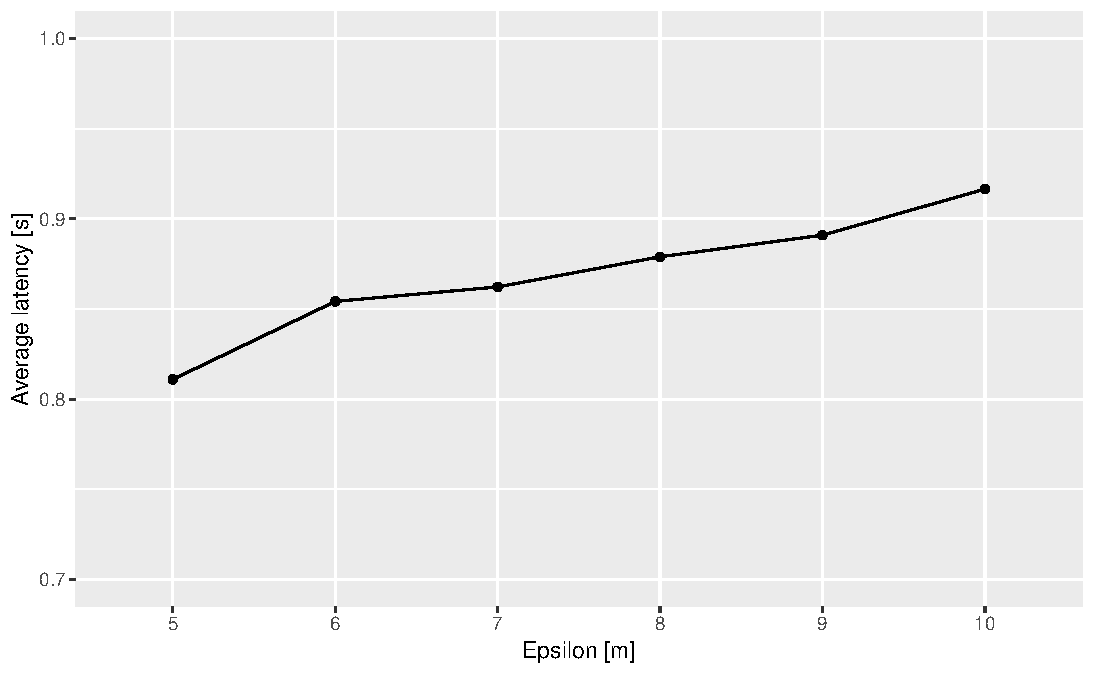
\includegraphics[width=\textwidth]{figures/LA_10K_MaximalsLatency}
            \caption{Latency.}
        \end{minipage}
        \hfill
        \begin{minipage}[b]{0.48\textwidth}
            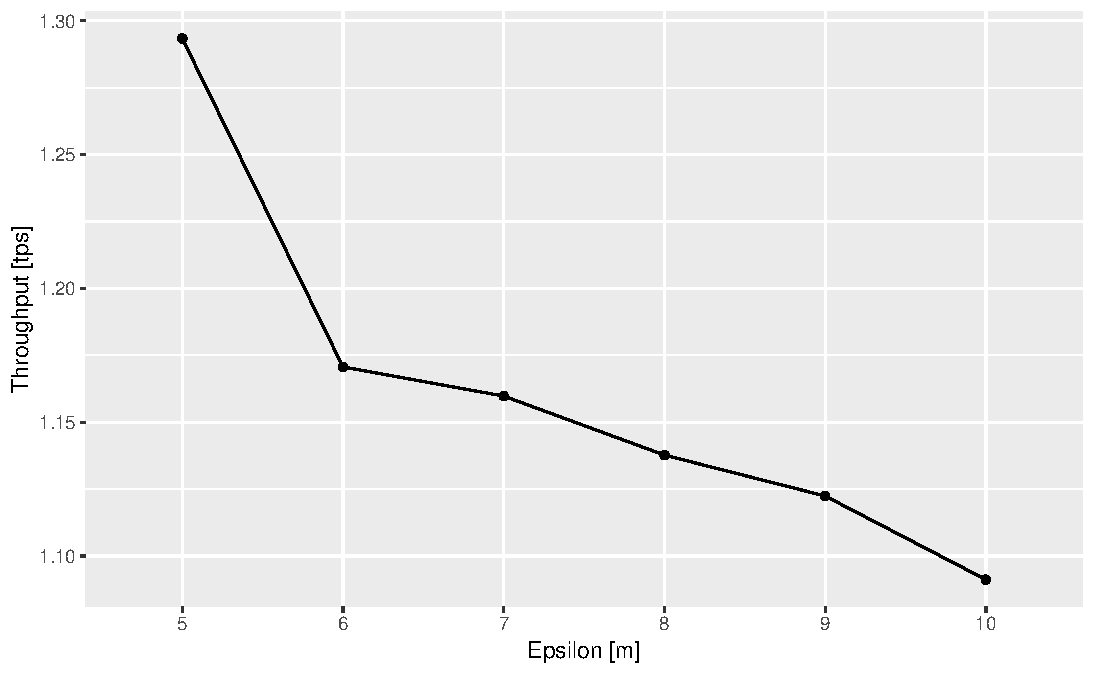
\includegraphics[width=\textwidth]{figures/LA_10K_MaximalsThroughput}
            \caption{Throughput.}
        \end{minipage}
    \end{figure}    
\end{frame}

\begin{frame}{LA\_10K Join consecutive time instants}
    \centering
    \begin{figure}
        \begin{minipage}[b]{0.48\textwidth}
            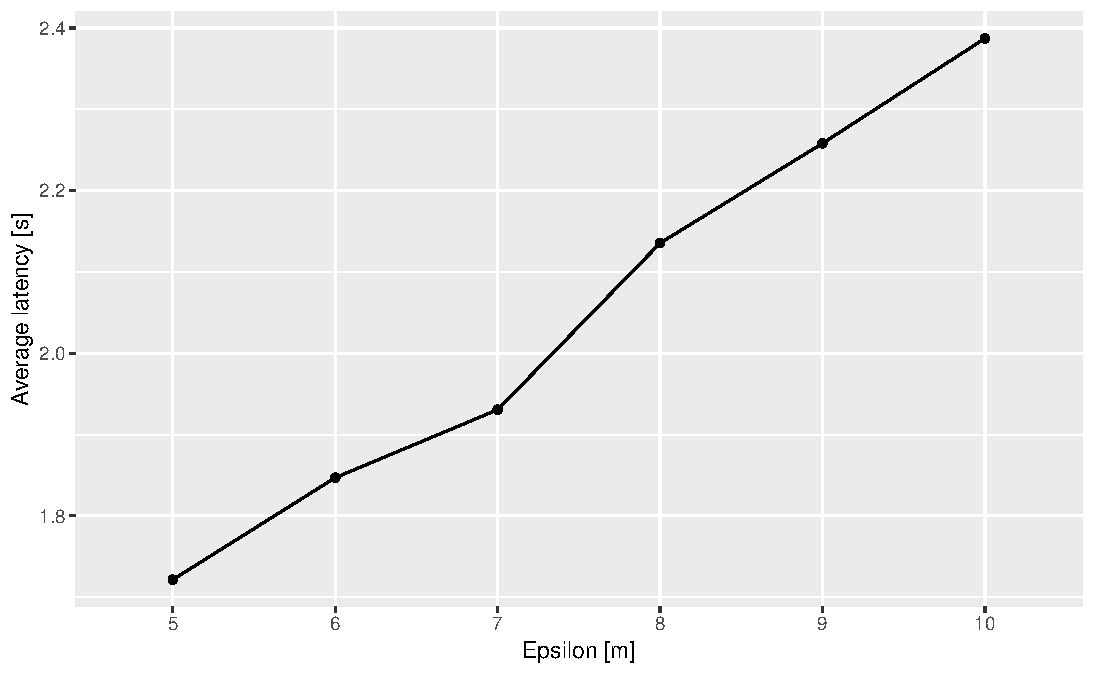
\includegraphics[width=\textwidth]{figures/LA_10K_JoinLatency}
            \caption{Latency.}
        \end{minipage}
        \hfill
        \begin{minipage}[b]{0.48\textwidth}
            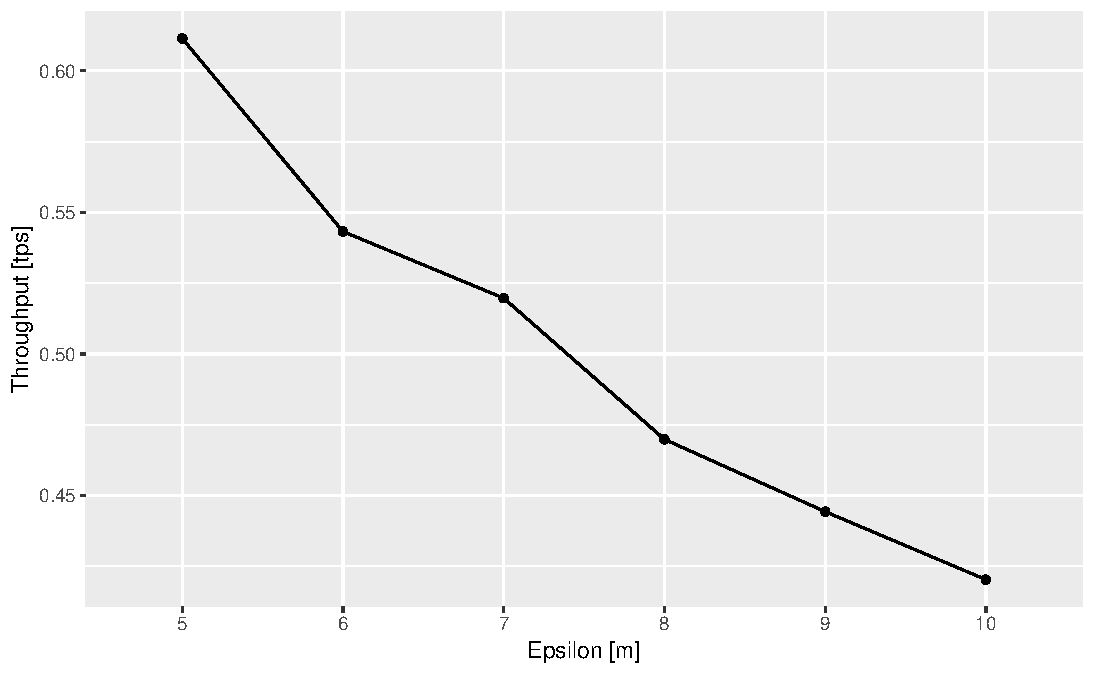
\includegraphics[width=\textwidth]{figures/LA_10K_JoinThroughput}
            \caption{Throughput.}
        \end{minipage}
    \end{figure}    
\end{frame}

\begin{frame}{LA\_5K Maximal disks finding}
    $\mu=5, \delta=15$.\\
    \blfootnote{Number of flocks: 225}
    \centering
    \begin{figure}
        \begin{minipage}[b]{0.48\textwidth}
            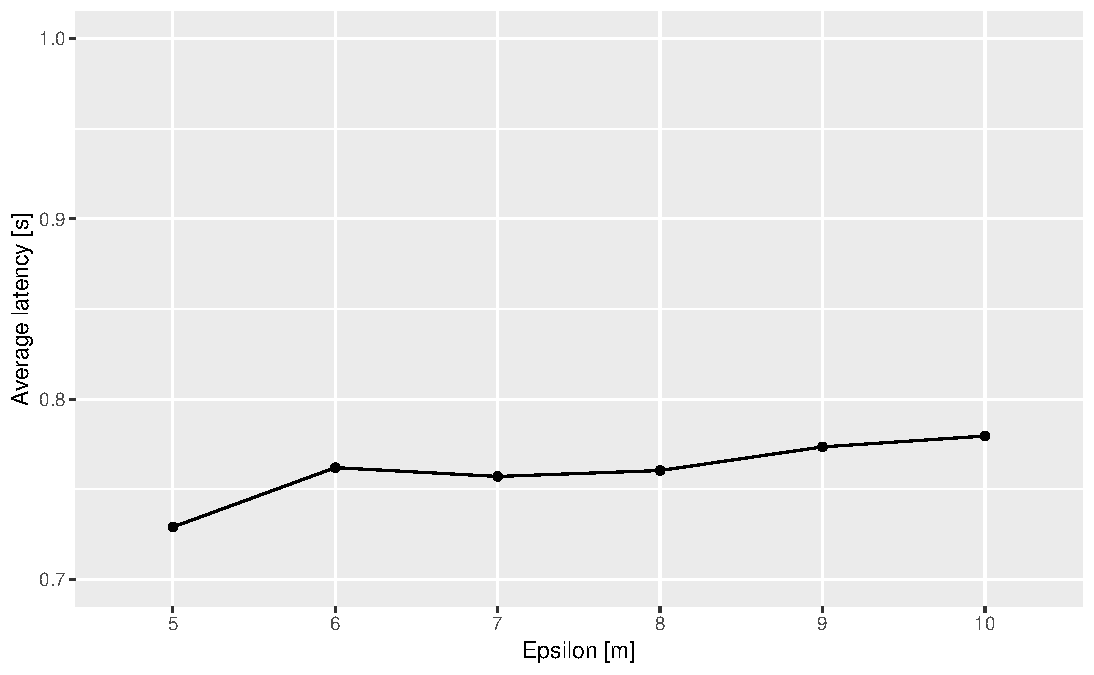
\includegraphics[width=\textwidth]{figures/LA_5K_MaximalsLatency}
            \caption{Latency.}
        \end{minipage}
        \hfill
        \begin{minipage}[b]{0.48\textwidth}
            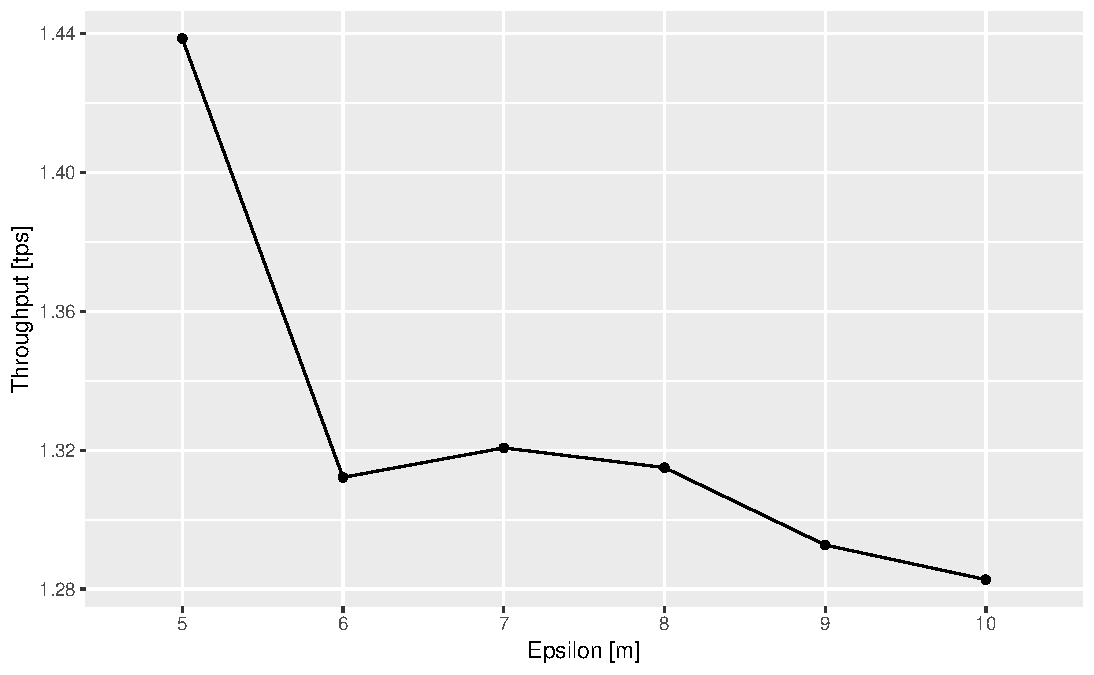
\includegraphics[width=\textwidth]{figures/LA_5K_MaximalsThroughput}
            \caption{Throughput.}
        \end{minipage}
    \end{figure}    
\end{frame}

\begin{frame}{LA\_5K Join consecutive time instants}
    \centering
    \begin{figure}
        \begin{minipage}[b]{0.48\textwidth}
            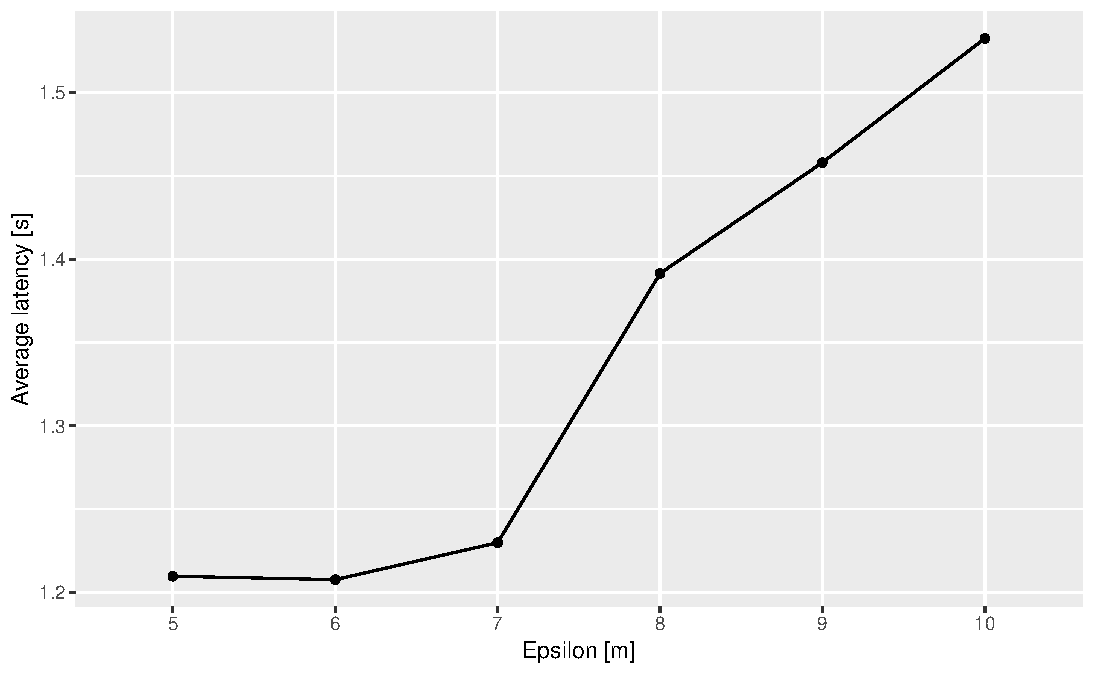
\includegraphics[width=\textwidth]{figures/LA_5K_JoinLatency}
            \caption{Latency.}
        \end{minipage}
        \hfill
        \begin{minipage}[b]{0.48\textwidth}
            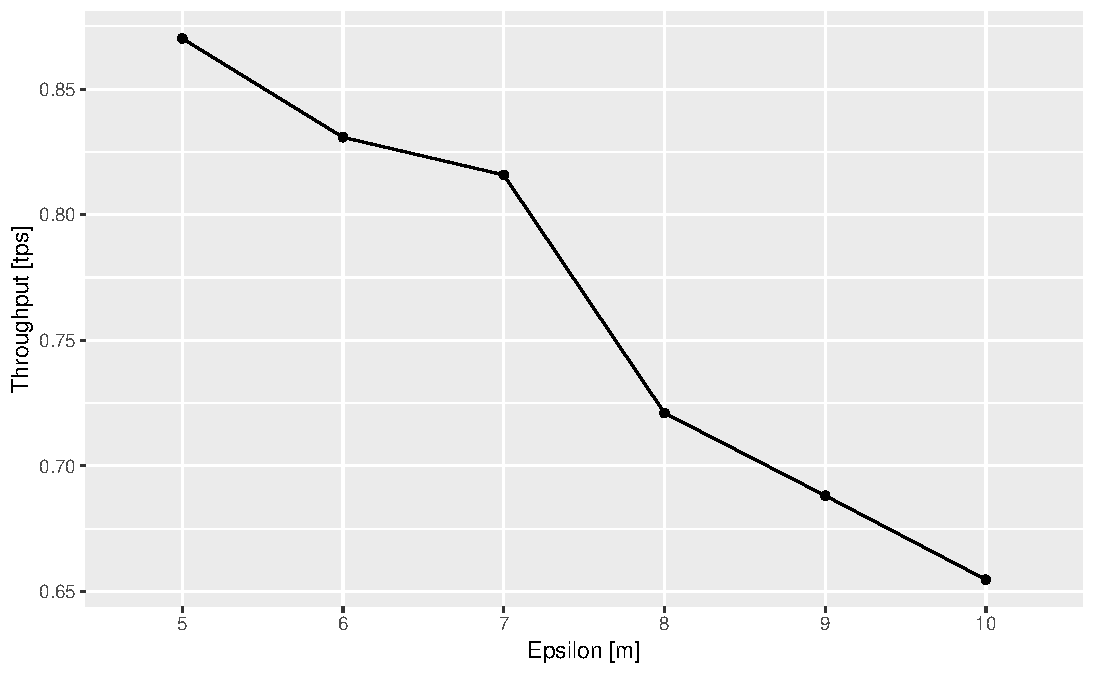
\includegraphics[width=\textwidth]{figures/LA_5K_JoinThroughput}
            \caption{Throughput.}
        \end{minipage}
    \end{figure}    
\end{frame}

\begin{frame}{Some remarks}
    \begin{itemize}
        \item Optimal number of partitions is small ($\approx 24$) due to the relatively small number of trajectories. It does not exploit all of the available cores.
        \item Chen et.al. (2019) exploits parallelism by mining several ($\eta$) snapshots at a time.
    \end{itemize}
\end{frame}

\begin{frame}{Issues with GeoLife dataset}
    \begin{itemize}
        \item I got the same number as Table 2 in Chen et.al. (2019), but the number of snapshots (92,645) is actually the number of snapshots for the longest trajectory.
        \item The real life span of the dataset is huge (170'985.600 snapshots).
        \item If any aggregation/interpolation is done the maximum number of moving objects at the same time is only 20, Actually the maximum number of users in the dataset is 182.
        \item In the last email, Dr Chen confirms that the $\epsilon$ value ranges between 8.2Km and 49.5Km.
    \end{itemize}
\end{frame}

\end{document}
